%% =============================================================
%%  IEEE Signal Processing Letters submission (5-page limit)
%%  Official IEEE SPL template structure with authors' original content
%% =============================================================
\documentclass[journal]{IEEEtran}

% ----- Graphics (from official template, PDF-aware) -----
\ifCLASSINFOpdf
  \usepackage[pdftex]{graphicx}
\else
  \usepackage[dvips]{graphicx}
\fi

% ----- URL and hyphenation (from official template) -----
\usepackage{url}
\hyphenation{op-tical net-works semi-conduc-tor}

% ----- Additional packages (from authors' file; algorithmic removed) -----
\usepackage{cite}
\usepackage{amsmath,amssymb,amsfonts}
\usepackage{textcomp}
\usepackage{xcolor}
\usepackage{booktabs}
\usepackage{multirow}
\usepackage{bm}

% ----- Math shortcuts -----
\newcommand{\vx}{\mathbf{x}}
\newcommand{\vr}{\mathbf{r}}
\DeclareMathOperator*{\argmin}{arg\,min}

\newcommand{\new}[1]{\textcolor{red}{#1}}  % CHANGED: blue -> red, marks revision edits

\def\ourmodel{SA-INR}

\begin{document}

% ============ Title ============
\title{Scattering-Aware Implicit Neural Representation for CT Metal Artifact Reduction}

% ============ Authors ============
% TODO: Update author affiliations and order
\author{
Ruibo~Wang,~Ziyi~Shen,~Junran~Yang,~Zhangling~Chen,~Ce~Wang,~Dong~Liang,~\IEEEmembership{Senior Member, IEEE}~and~Kun~Shang
\thanks{This study was supported in part by the National Natural Science Foundation of China (No. 62301532 and 62201384), and in part by the Natural Science Foundation of Shenzhen City (No. JCYJ20230807140601003).}
\thanks{Ruibo~Wang is with the Faculty of Electrical Engineering, Mathematics and Computer Science, Delft University of Technology, 2600 AA Delft, Netherlands.}
\thanks{Ziyi~Shen and Dong~Liang are with School of Biomedical Engineering, Southern Medical University, Guangzhou, Guangdong 510515, China.}
\thanks{Junran~Yang is with school of Artificial Intelligence, Tianjin university, Tianjin 300387, China.}
\thanks{Zhangling~Chen is with School of Mathematical Sciences, Tianjin Normal University, Tianjin 300387, China.}
\thanks{Ce~Wang is with the School of science, Sun Yat-sen University, Shenzhen, 518107, Guangdong province, China.}
\thanks{Dong~Liang and Kun~Shang are with Research Center for BCI, Shenzhen Institutes of Advanced Technology, Chinese Academy of Sciences, Shenzhen, Guangdong, China. And he is also with Guangdong Provincial Key Laboratory of Multimodality Non-Invasive Brain-Computer Interfaces, Shenzhen, Guangdong, China.}
\thanks{Corresponding authors are Dong~Liang and Kun~Shang. E-mail: dong.liang@siat.ac.cn; kunzzz.shang@gmail.com}
\thanks{\new{Code and trained models are available at https://github.com/WRBcode/SA-INR\,.}}
}
\markboth{Journal of \LaTeX\ Class Files, Vol. 14, No. 8, August 2015}
{Wang \MakeLowercase{\textit{et al.}}: \ourmodel : Physics-Informed CT MAR via PTE and INR}
\maketitle

% ============ Abstract ============
\begin{abstract}
Implicit neural representation (INR) has emerged as a promising unsupervised solution to CT metal artifact reduction (MAR). However, residual halo artifacts often persist near metallic implants because attenuation-only forward models neglect in-scatter and thus introduce a systematic forward-model mismatch. In this letter, we propose \ourmodel, a scattering-aware INR framework that augments the conventional polychromatic attenuation model with a lightweight in-scatter correction inspired by the photon transport equation. SA-INR admits both a physics-constrained version and a learnable version, enabling a trade-off between interpretability and flexibility. Experiments on DeepLesion show that \ourmodel\ improves MAR quality and robustness. Notably, the physics-constrained version improves over the state-of-the-art INR baseline without introducing additional trainable parameters, while the learnable version achieves the best overall performance (34.37\,dB PSNR, 0.9499 SSIM). \new{A capacity-matched ablation further confirms that the gain stems from the scattering-aware prior rather than from additional learnable parameters.} Ablation studies further show that a strongly forward-peaked scattering prior is essential for stable optimization. These results indicate that modest but physically structured forward-model corrections can improve both reconstruction quality and robustness in unsupervised INR-based CT MAR.
\end{abstract}

% ============ Index Terms ============
\begin{IEEEkeywords}
Metal artifact reduction, computed tomography, implicit neural representations, photon transport equation, scattering-aware MAR.
\end{IEEEkeywords}

\section{Introduction}
\IEEEPARstart{C}{omputed} tomography (CT) is widely used in clinical diagnosis~\cite{hsieh2003computed}, yet metallic implants often cause severe streak and halo artifacts arising from nonlinear effects such as beam hardening, photon starvation, and scattering, which violate standard reconstruction assumptions and degrade diagnostic image quality~\cite{meyer2010normalized, gjesteby2016metal}.

Existing metal artifact reduction (MAR) methods can be broadly grouped into three categories. \textit{Classical model-based methods}~\cite{kalender1987reduction, meyer2010normalized, mehranian2013x} typically treat metal-corrupted sinogram measurements as missing data and restore them using interpolation or handcrafted priors, but often introduce secondary artifacts because projection consistency is only approximately enforced. \textit{Supervised methods}~\cite{zhang2018convolutional, lin2019dudonet, wang2021indudonet, su2024f2iflow, baoshun2024artifact} achieve strong performance through data-driven priors, yet require large-scale paired training data and often suffer from limited out-of-domain generalization in clinical deployment~\cite{liao2019adn, song2022solving}. \new{Recent supervised work explores complementary directions including global-context Transformers~\cite{baoshun2024artifact}, hybrid model-/data-driven coupling~\cite{shi2024coupling}, prompt-guided universal MAR~\cite{shi2025visual}, and optimization-inspired designs beyond unfolding~\cite{jiang2025optnet}, further illustrating the breadth of supervised MAR research.} More recently, \textit{unsupervised methods} that optimize directly from the measured scan have emerged as an attractive alternative~\cite{baguer2020computed, chen2025unsupervised}. Among them, \textit{implicit neural representation} (INR) methods~\cite{shen2022nerp} model the attenuation field as a coordinate-based neural network optimized per scan. Recent methods such as Polyner~\cite{wu2023unsupervised} further incorporate polychromatic attenuation and better address beam hardening. However, current INR-based CT forward models remain largely attenuation-driven and typically omit explicit correction for in-scatter, i.e., photons scattered into the detector from off-axis directions.

Omitting in-scatter introduces a systematic forward-model mismatch in metal-affected regions. As illustrated in Fig.~\ref{fig:toy}, the measured detector signal along a ray $\vr$ traversing metal may contain both directly transmitted photons $L_{\mu}$ and in-scattered photons $L_{\text{is}}$, i.e., $L_{\text{total}} = L_{\mu} + L_{\text{is}}$. In contrast, an attenuation-only forward model predicts only $L_{\mu}$, yielding $L_{\text{pred}} = L_{\mu} < L_{\text{total}}$. To reduce this discrepancy, the estimated attenuation along the ray tends to be lowered during optimization, which in turn leads to attenuation underestimation near metal boundaries and residual bright halo artifacts. This observation suggests that part of the residual error in INR-based CT MAR arises from forward-model mismatch, motivating a scattering-aware correction in the forward process.

\begin{figure}[t!]
\centering
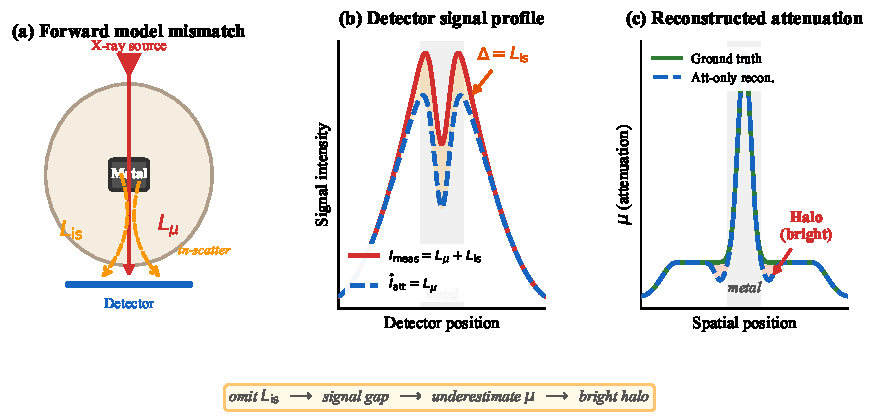
\includegraphics[width=0.92\columnwidth]{fig_toy_example.pdf}
\caption{Toy example illustrating the forward-model mismatch caused by omitting in-scatter. \textbf{(a)} A ray traversing metal contains both directly transmitted photons $L_{\mu}$ and in-scattered photons $L_{\text{is}}$. \textbf{(b)} The attenuation-only prediction (dashed) underestimates the measured detector signal (solid) in the metal-affected region. \textbf{(c)} To reduce this discrepancy, the optimizer lowers $\mu$ near the metal boundary, leading to bright halo artifacts.}
\label{fig:toy}
\vspace{-3mm}
\end{figure}

To address this issue, we propose a scattering-aware INR framework, termed \ourmodel, that augments the conventional attenuation-only forward model with a lightweight in-scatter correction inspired by the photon transport equation (PTE). Rather than solving the full PTE, \ourmodel introduces a differentiable approximation that captures the dominant forward-scattering effect overlooked by existing INR-based MAR methods. The proposed framework can be implemented either as a physics-constrained variant or as a lightweight learnable variant, offering a flexible trade-off between accuracy and efficiency. The main contributions of this work are as follows. 
\begin{enumerate}
  \item We identify a forward-model mismatch in INR-based CT-MAR arising from the omission of in-scatter, and analyze its role in producing residual halo artifacts.
  \item We propose \ourmodel, a scattering-aware INR framework that incorporates a lightweight in-scatter correction, which can be implemented as either a physics-constrained or a learnable variant.
  \item Experimental results, together with ablation analyses, demonstrate that a strongly forward-peaked scattering prior is critical for stable optimization and improved reconstruction quality.
\end{enumerate}

\section{Method}

\begin{figure}[t!]
\centering
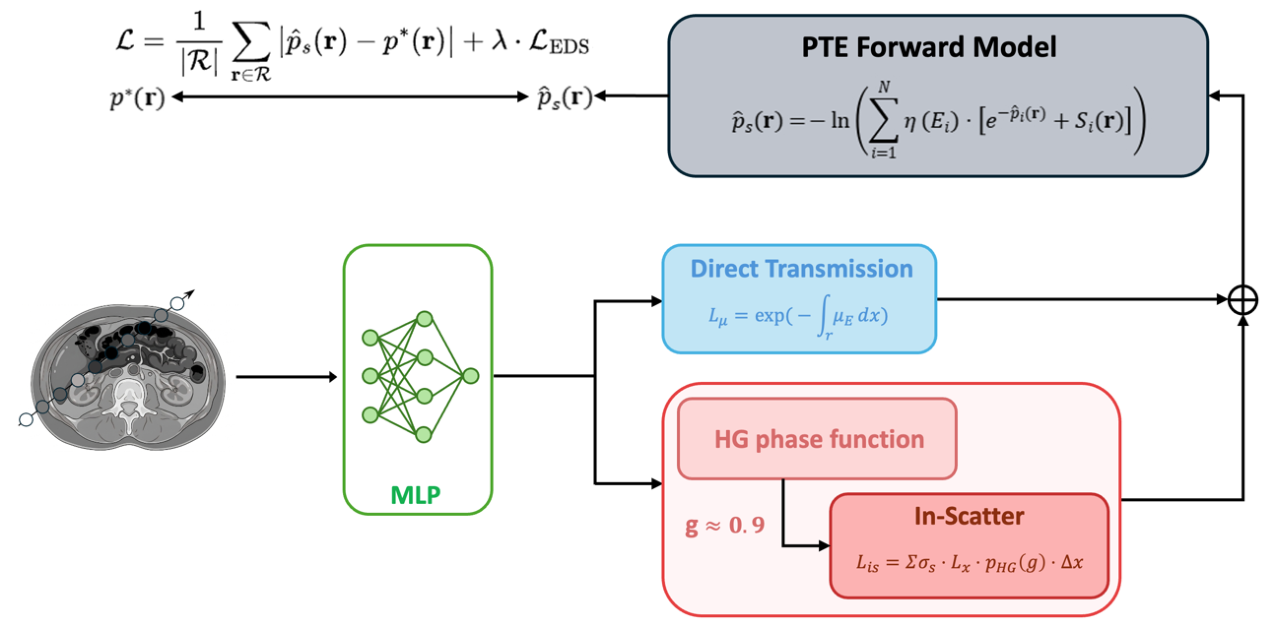
\includegraphics[width=0.75\columnwidth]{fig_main.pdf}
\caption{Overview of the proposed \ourmodel\ framework. Given ray sample coordinates, an MLP predicts energy-dependent attenuation coefficients and passes them through a direct transmission branch and a scattering-aware correction branch. The two components are then combined in the final forward model to synthesize projections for optimization against the measured sinogram.}\label{fig:pipeline}
\vspace{-3mm}
\end{figure}

\subsection{Attenuation-Only INR Forward Model}
We first review the attenuation-only forward model used in existing INR-based CT reconstruction methods, which typically synthesize projections using the polychromatic Beer-Lambert law:
\begin{equation}\label{eq:polyner}
 p(\vr) = -\ln \int \eta(E)\cdot \exp\!\left(-\int_{\vr}\mu_E(\vx)\,d\ell\right)dE,
\end{equation}
where $\eta(E)$ denotes the source spectrum and $\mu_E(\vx)$ is the energy-dependent linear attenuation coefficient at spatial location $\vx$.

While this formulation alleviates beam-hardening effects, it remains absorption-driven and omits in-scatter. When in-scatter is non-negligible, the predicted projections fall systematically below the measurements near metallic implants, and the INR compensates by underestimating local attenuation, manifesting as residual bright halo artifacts. This motivates a scattering-aware correction in the forward model.

\subsection{Scattering-Aware Forward Model}
To overcome the forward-model mismatch discussed above, we introduce \ourmodel, a scattering-aware INR framework that augments the conventional attenuation-only formulation with an explicit in-scatter term, as illustrated in Fig.~\ref{fig:pipeline}. 
Given the attenuation field predicted by the INR, the detector signal is modeled as the sum of direct transmission and in-scatter contributions:
\begin{equation}\label{eq:pte}
  L_{\text{total}}(\vr)=L_{\mu}(\vr)+L_{\text{is}}(\vr).
\end{equation}

Rather than solving the full PTE, we adopt a lightweight differentiable approximation to capture the dominant forward-scattering effect. The angular distribution of scattered photons is modeled using the Henyey-Greenstein (HG) phase function:
\begin{equation}\label{eq:hg}
  p_{\text{HG}}(\cos\theta;g)=\frac{1-g^2}{4\pi(1+g^2-2g\cos\theta)^{3/2}},
\end{equation}
where $g\in[-1,1]$ is the anisotropy factor. Under strong forward peaking ($g \approx 0.9$), the dominant contribution comes from near-forward scattering, motivating a single-scattering approximation of the full transport process that retains the main correction needed for metal-affected projections.

\new{This approximation makes three simplifications relative to a full PTE solution: (i) \emph{single-scattering}, ignoring multiple-scattering paths, which is reasonable in the strongly forward-peaked regime where the leading term dominates near the metal--tissue interface; (ii) a fixed \emph{forward direction} $\cos\theta{=}1$ as a tractable surrogate for the angular integral, well justified at large $g$ but degrading as $g\rightarrow0$; and (iii) an \emph{energy-independent angular kernel}, with material dependence absorbed into the per-region albedo. Our formulation is thus a physically structured projection-domain correction rather than a substitute for solving the PTE; Monte Carlo or multi-order PTE solvers are left as future work.}

\subsection{Differentiable Ray Marching Formulation}
For efficient end-to-end optimization, we discretize the forward process along each ray $\vr$ using $N_s$ sample points. \new{Throughout this subsection, $N_s$ denotes the number of sample points along a ray, while $N$ denotes the number of discrete energy bins (introduced in Sec.~II-D). Both indices are reserved to avoid ambiguity.}

\textbf{1) Scattering coefficient.}
At the $n$-th sample point, the effective scattering coefficient is defined as
\begin{equation}
\sigma_s(n)=a(n)\mu_E(\vx_n),
\end{equation}
where $a(n)$ is the local \new{(dimensionless)} albedo and $\mu_E(\vx_n)$ is the energy-dependent linear attenuation coefficient \new{(unit: cm$^{-1}$)} predicted by the MLP at sample point $\vx_n$. \new{Consequently $\sigma_s$ shares the same units as $\mu_E$. The albedo $a(n)$ takes one of two material-dependent values, $(a_{\text{metal}}, a_{\text{tissue}})$, selected by the metal mask $\mathcal{M}$ defined below.}

\textbf{2) Direct transmission.}
The discrete direct transmission term at the $n$-th sample point is
\begin{equation}\label{eq:transmit}
  L_\mu(n)=I_0\exp\!\left(-\sum_{k=1}^{n}\mu_E(\vx_k)\Delta x\right),
\end{equation}
where $I_0$ is the source intensity \new{(normalized to $I_0{=}1$, so that $L_\mu(n)\in(0,1]$ lies in the same normalized detector-intensity domain as $e^{-\hat{p}_i}$ in Eq.~\eqref{eq:final})} and $\Delta x$ is the sampling interval.

\textbf{3) Per-point scattering contribution.}
The scattering contribution generated at the $n$-th sample point is approximated by
\begin{equation}\label{eq:scatter_n}
  S_{\text{cont}}(n)=\sigma_s(n)L_\mu(n)p_{\text{HG}}(1.0;g)\Delta x,
\end{equation}
where $\cos\theta=1$ is used to approximate the dominant forward-scattering component. \new{Here $p_{\text{HG}}$ is used as a relative angular weight, with its solid-angle factor (sr$^{-1}$) absorbed into the dimensionless albedo and the overall normalization, so that $S_{\text{cont}}(n)$ remains on the same normalized intensity scale as $L_\mu$.}

\textbf{4) Ray-wise aggregation.}
The total scattering contribution for energy bin $i$ along ray $\vr$ is
\begin{equation}\label{eq:scatter_total}
  S_i(\vr)=\sum_{n=1}^{N_s}S_{\text{cont}}^{(i)}(n),
\end{equation}
\new{where $S_{\text{cont}}^{(i)}(n)$ denotes the per-point scattering contribution of Eq.~\eqref{eq:scatter_n} evaluated at energy bin $E_i$ (i.e.\ replacing $\mu_E$ and $\sigma_s$ by their values at $E_i$). The summation is taken in the detector-intensity domain, so $S_i(\vr)$ shares the same units as $e^{-\hat{p}_i(\vr)}$ and can be added to it directly in Eq.~\eqref{eq:final}.}

\subsection{Final Forward Projection and Optimization}
The final polychromatic forward model with scattering correction is defined as
\begin{equation}\label{eq:final}
  \hat{p}_s(\vr)=-\ln\!\left(\sum_{i=1}^{N}\eta(E_i)\left[e^{-\hat{p}_i(\vr)}+S_i(\vr)\right]\right),
\end{equation}
where $\hat{p}_i(\vr)$ denotes the attenuation-only projection at energy $E_i$ and $N$ is the number of discrete energy bins. \new{Here $e^{-\hat{p}_i(\vr)}\in(0,1]$ is the transmission fraction, and $S_i(\vr) \geq 0$ is the per-bin scattered intensity, normalized by the source intensity $I_0$ to be dimensionless and scale-consistent with the transmission term. The spectrum $\eta(E_i)$ is normalized to $\sum_i \eta(E_i)=1$, so the bracketed sum is a convex combination across energy bins.}
The network is optimized end-to-end by minimizing
\begin{equation}\label{eq:loss}
  \mathcal{L}=\frac{1}{|\mathcal{R}|}\sum_{\vr\in\mathcal{R}}\left|\hat{p}_s(\vr)-p^*(\vr)\right|+\lambda\mathcal{L}_{\text{EDS}},
\end{equation}
where $p^*(\vr)$ is the measured sinogram and $\mathcal{L}_{\text{EDS}}$ is the energy-dependent smoothness regularizer following~\cite{wu2023unsupervised}, defined as
\begin{equation}\label{eq:eds}
\mathcal{L}_{\text{EDS}} = \frac{1}{|\mathcal{R}||\vr|}\sum_{\vr\in\mathcal{R}}\sum_{\vx\in\vr}[1-\mathcal{M}(\vx)]\sum_{i=2}^{N}\left|\mu_{E_i}(\vx)-\mu_{E_{i-1}}(\vx)\right|,
\end{equation}
which enforces smooth variation of the predicted attenuation across adjacent energy levels in non-metal regions ($\mathcal{M}(\vx){=}0$). The weight $\lambda{=}0.2$ balances data fidelity and regularization.

\new{The binary metal mask $\mathcal{M}(\vx)\in\{0,1\}$ is obtained by thresholding the filtered back-projection (FBP) reconstruction of the metal-corrupted sinogram with a fixed HU threshold of $2500$~HU (i.e.\ pixels above the threshold are labeled as metal, $\mathcal{M}=1$) and then morphologically padded to the reconstruction grid. The same FBP-based mask is used to (i) gate the EDS regularizer above and (ii) select the per-sample albedo $(a_{\text{metal}}, a_{\text{tissue}})$ at training time.}

The scattering module is implemented in two forms. The physics-constrained version (\ourmodel-P) uses fixed HG-based scattering with $g=0.9$ and fixed albedo values \new{($a_{\text{metal}}=0.5$, $a_{\text{tissue}}=0.9$), motivated by the NIST scattering tables for typical metallic implants vs. soft tissue at diagnostic energies}. The learnable version (\ourmodel-L) replaces the analytic scatter term with a lightweight MLP-based correction. This design allows us to separate the effect of the scattering-aware prior from that of additional learnable flexibility.

\new{\textbf{SA-INR-L module specification.} The scattering branch of \ourmodel-L is a 3-layer MLP ($\mathbb{R}^2\!\rightarrow\!64\!\rightarrow\!64\!\rightarrow\!1$, ReLU hidden activations with a Softplus output that enforces non-negativity, $\approx$4.4k params, Kaiming-uniform init) that takes the same 2D coordinate $\vx_n$ as the hash-grid INR and outputs a non-negative per-sample modulation shared across all $N{=}100$ energy bins. The fixed albedos are replaced by two learnable scalars $\alpha_{\text{metal}},\alpha_{\text{tissue}}$ initialized at $(0.5,0.9)$. All parameters (INR, scattering MLP, albedos) are optimized jointly by a single Adam optimizer with the same learning rate/schedule.}

\section{Experiments}
\subsection{Setup}
We evaluate the proposed method on the DeepLesion dataset~\cite{yan2018deeplesion} with simulated metal artifacts following~\cite{wu2023unsupervised}. A total of 200 CT slices of size $256\times256$ are selected, and each slice is embedded with a randomly chosen metal mask from a clinical implant library. Polychromatic forward projections are synthesized using a 120\,kVp GE spectrum (20--120\,keV) under a fan-beam geometry with 360 views and 611 detectors. Poisson noise and beam-hardening correction are applied.

To isolate the effect of the proposed forward-model correction, we adopt the same network architecture and training protocol as Polyner~\cite{wu2023unsupervised}. The attenuation field is represented by a hash-grid encoded MLP~\cite{muller2022instant} and optimized independently for each slice. The loss consists of an $L_1$ data-fidelity term and an energy-dependent smoothness regularizer with $\lambda=0.2$. Following prior MAR evaluation practice, PSNR and SSIM are computed on non-metal regions.

\new{\textbf{Training details.} Per-scan settings: Adam, learning rate $10^{-3}$ with step decay (factor $0.1$), $4000$ epochs per slice, ray batch $16000$ ($2$ samples/view), $N{=}100$ energy bins (20--120\,keV), $\lambda{=}0.2$. The hash-grid encoder ($16$ levels, $8$ features/level, $\log_2$ hashmap $19$) feeds a fully-fused MLP ($2$ hidden layers, width $128$, Softplus output). All runs use a single NVIDIA RTX A6000 (48\,GB).}

\subsection{Quantitative Results}
\begin{table}[t!]
  \centering
  \caption{Reconstruction accuracy and robustness on 200 DeepLesion test slices.}
  \label{tab:results}
  \begin{tabular}{@{}lcclc@{}}
    \toprule
    Method & PSNR (dB) & SSIM  &Memory & \new{Time/slice}\\
    \midrule
    FBP     & 29.14$\pm$3.26 & 0.7201$\pm$0.111  &2\,MiB& ~0.1s\\
    LI-MAR  & 31.05$\pm$2.54 & 0.8284$\pm$0.058  &3\,MiB& ~1s\\
    NMAR    & 32.12$\pm$2.60 & 0.8555$\pm$0.060  &5\,MiB& ~2s\\
    \midrule
    Polyner & 34.02$\pm$1.79 & 0.9473$\pm$0.022  &3360\,MiB & 3.5min\\
    \new{Polyner-Cap}& \new{33.90$\pm$0.93}& \new{0.7977$\pm$0.045}&\new{4173\,MiB} & \new{4.1min}\\
 \ourmodel-P & 34.15$\pm$1.56 & 0.9481$\pm$0.025  & 4173\,MiB &4.1min\\
    \textbf{\ourmodel-L} & \textbf{34.37$\pm$1.41} & \textbf{0.9499$\pm$0.014}  &5955\,MiB & 6 min\\
    \bottomrule
  \end{tabular}
\end{table}

Table~\ref{tab:results} compares \ourmodel against classical baselines and Polyner. \ourmodel-P achieves higher PSNR than Polyner without additional trainable parameters, showing the gain stems from the scattering-aware correction rather than capacity. \ourmodel-L performs best, with the highest mean PSNR/SSIM and the lowest variance; the reduced variance indicates more consistent reconstruction across diverse metal configurations, important in unsupervised per-scan optimization. 


\new{\textbf{Capacity-matched control.} To confirm the gain is not merely from extra parameters, we train \emph{Polyner-Cap}: a Polyner backbone with an auxiliary MLP of the same size as the \ourmodel-L scattering branch ($2\!\rightarrow\!64\!\rightarrow\!64\!\rightarrow\!1$, $\sim$4.4k params) plus the two learnable scalars, but \emph{without} the HG phase or transmittance/$\sigma_s$ aggregation (a free per-ray correction), trained with the same optimizer, learning rate, and number of epochs for a fair comparison. As shown in Table~\ref{tab:results}, Polyner-Cap matches Polyner in PSNR ($34.02$ vs.\ $33.90$~dB) yet its SSIM drops sharply to $0.7977$: an unconstrained MLP absorbs projection residuals without being tied to the attenuation field, hurting perceptual consistency. Added capacity alone therefore does not help and can even degrade structural fidelity; the advantage of \ourmodel stems from the scattering-aware structural prior rather than from extra parameters.}

The two versions also offer an accuracy-efficiency trade-off: \ourmodel-P adds only moderate memory while preserving parameter efficiency, whereas \ourmodel-L attains the best performance at higher cost. 

\subsection{Qualitative Analysis}
Fig.~\ref{fig:visual} compares a representative test slice with zoomed ROIs and error maps near the metal boundary. Classical MAR methods suppress major streaks but introduce secondary artifacts and blurring, and Polyner still exhibits residual halo-like errors near metal. In contrast, \ourmodel consistently suppresses these metal-adjacent residual artifacts while better preserving surrounding anatomical structures.

\begin{figure}[!t]
\centering
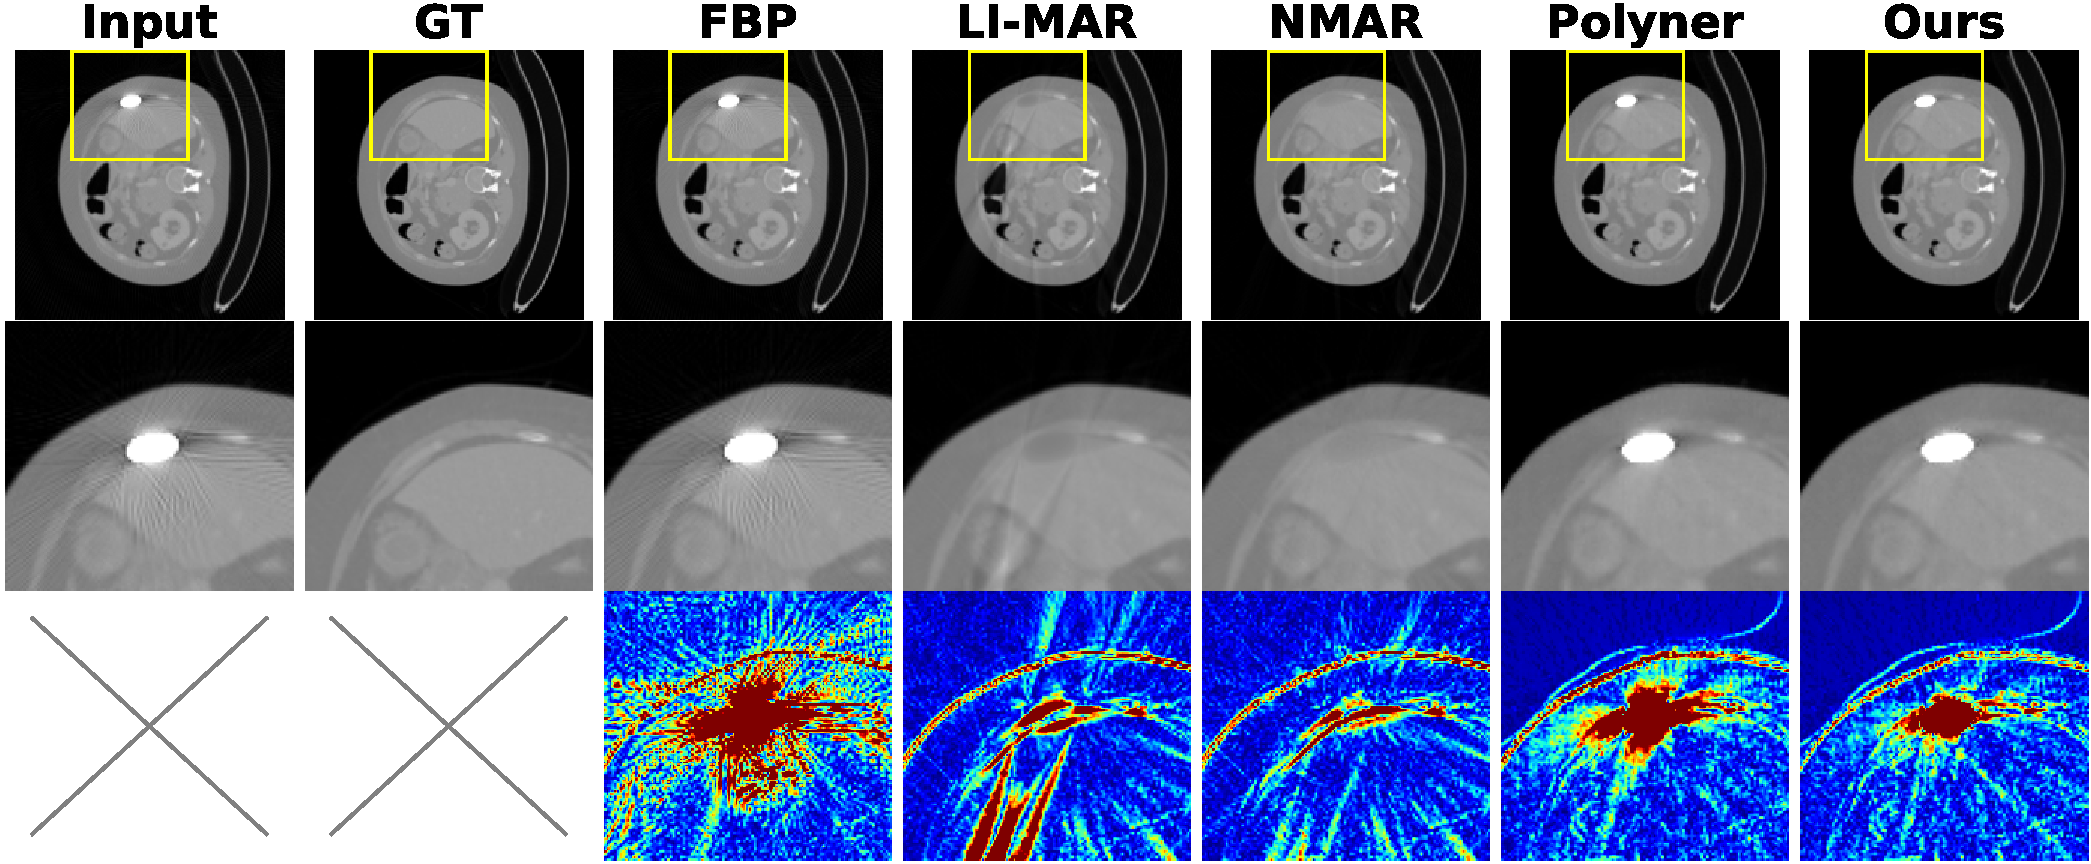
\includegraphics[width=7.2cm]{fig_comparison_case6_0313_big.pdf}
\caption{Visual comparison on a representative test slice (with zoomed ROIs and error maps near the metal boundary). From left to right: ground truth, metal-corrupted input, classical MAR methods, Polyner, and the proposed method. The proposed method reduces residual halo artifacts near the implant and yields lower reconstruction error.}
\label{fig:visual}
\vspace{-3mm}
\end{figure}


\subsection{Ablation Studies}

\begin{table}[t!]
  \centering
  \caption{Ablation studies on the anisotropy factor $g$ (top) and albedo assignment (bottom). The $g{=}0.9$ and $(0.5,0.9)$ rows denote the same configuration (\ourmodel-P).}
  \label{tab:ablation}
  \small\setlength{\tabcolsep}{4pt}\renewcommand{\arraystretch}{0.9}
  \begin{tabular}{@{}lccc@{}}
    \toprule
    Setting & PSNR (dB) & SSIM & Note \\
    \midrule
    \multicolumn{4}{@{}l}{\textit{Anisotropy} $g$ (albedo fixed at NIST $(0.5,0.9)$):}\\
    $g{=}0.0$  & diverged & --- & \texttimes \\
    $g{=}0.5$  & 32.41$\pm$5.14 & 0.9136$\pm$0.085 & $\triangle$ \\
    $g{=}0.7$  & 32.73$\pm$5.39 & 0.9176$\pm$0.100 & $\triangle$ \\
    \textbf{$g{=}0.9$} & \textbf{34.15$\pm$1.56} & \textbf{0.9481$\pm$0.025} & \checkmark \\
    $g{=}0.95$ & 34.15$\pm$2.07 & 0.9461$\pm$0.035 & \checkmark \\
    \midrule
    \multicolumn{4}{@{}l}{\textit{Albedo} $(a_{\text{metal}},a_{\text{tissue}})$ (at $g{=}0.9$):}\\
    (0, 0)       & 34.02$\pm$1.79 & 0.9473$\pm$0.022 & No scatter \\
    (0.3, 0.3)   & 32.74$\pm$4.52 & 0.9179$\pm$0.076 & Uniform low \\
    (0.9, 0.9)   & 33.56$\pm$3.08 & 0.9316$\pm$0.049 & Uniform high \\
    (0.9, 0.5)   & 32.25$\pm$6.64 & 0.9112$\pm$0.109 & Inverted \\
    \textbf{(0.5, 0.9)} & \new{\textbf{34.15$\pm$1.56}} & \new{\textbf{0.9481$\pm$0.025}} & NIST (best) \\
    \bottomrule
  \end{tabular}
\end{table}

Table~\ref{tab:ablation} evaluates the HG anisotropy factor $g$. Isotropic or weakly anisotropic settings lead to unstable training or large variance, whereas strongly forward-peaked settings yield both higher accuracy and better robustness. The improvement depends not on simply adding an auxiliary term, but on imposing a physically meaningful forward-scattering prior: appropriate forward-peaked assumptions stabilize training, while inappropriate ones destabilize it, indicating that the gain comes from the scattering-aware formulation rather than generic model flexibility.



The lower block of Table~\ref{tab:ablation} evaluates albedo sensitivity: uniform settings degrade accuracy and robustness, the inverted contrast is worst (largest variance, $std{=}6.64$), and the NIST-motivated $(0.5,0.9)$ is best, confirming the correction benefits from a physically plausible material-dependent prior.

\section{Discussion and Conclusion}

Our simulation uses a simplified scatter model, so the gains evidence the usefulness of a physically structured forward-model correction rather than exact scatter physics, and the correction may also absorb other unmodeled errors. Future work targets more realistic scatter modeling and clinical validation.


Overall, the physics-constrained SA-INR improves accuracy and robustness over the attenuation-only baseline without extra trainable parameters, while the learnable version performs best, showing that physically structured forward-model corrections benefit unsupervised INR-based CT-MAR.

% ============= REFERENCES =============
% NOTE: Keep references concise for 4-page limit. Target ~15 refs max.

\bibliographystyle{IEEEtran}
\bibliography{references}

\end{document} 